%% Version 5.0, 2 January 2020
%
%%%%%%%%%%%%%%%%%%%%%%%%%%%%%%%%%%%%%%%%%%%%%%%%%%%%%%%%%%%%%%%%%%%%%%
% TemplateV5.tex --  LaTeX-based template for submissions to the
% American Meteorological Society
%
%%%%%%%%%%%%%%%%%%%%%%%%%%%%%%%%%%%%%%%%%%%%%%%%%%%%%%%%%%%%%%%%%%%%%
% PREAMBLE
%%%%%%%%%%%%%%%%%%%%%%%%%%%%%%%%%%%%%%%%%%%%%%%%%%%%%%%%%%%%%%%%%%%%%

%% Start with one of the following:
% DOUBLE-SPACED VERSION FOR SUBMISSION TO THE AMS
\documentclass[]{ametsocV5}


% TWO-COLUMN JOURNAL PAGE LAYOUT---FOR AUTHOR USE ONLY
% \documentclass[twocol]{ametsocV5}


% Enter packages here. If too many math alphabets are used,
% remove unnecessary packages or define hmmax and bmmax as necessary.

\newcommand{\hmmax}{0}
\newcommand{\bmmax}{0}
\usepackage{amsmath,amsfonts,amssymb,bm}
\usepackage{mathptmx}%{times}
\usepackage{newtxtext}
\usepackage{newtxmath}

\usepackage{gensymb}
\usepackage{subfig}

%%%%%%%%%%%%%%%%%%%%%%%%%%%%%%%%

%%% To be entered by author:

%% May use \\ to break lines in title:

\title{Title here}


\authors{Elio Campitelli
\correspondingauthor{Elio Campitelli,elio.campitelli@cima.fcen.uba.ar}
and Leandro Díaz
}

\affiliation{CIMA UBA blablabla}

\extraauthor{Carolina Vera
}


%%%%%%%%%%%%%%%%%%%%%%%%%%%%%%%%%%%%%%%%%%%%%%%%%%%%%%%%%%%%%%%%%%%%%
% ABSTRACT
%
% Enter your abstract here
% Abstracts should not exceed 250 words in length!
%


\abstract{Enter the text of your abstract here. This is a sample American
Meteorological Society (AMS) \LaTeX~template. This document provides
authors with instructions on the use of the AMS \LaTeX~template. Authors
should refer to the file amspaper.tex to review the actual \LaTeX~code
used to create this document. The template.tex file should be modified
by authors for their own manuscript.}

\begin{document}

%% Necessary!
\maketitle

\bibliographystyle{ametsoc2014}
%%%%%%%%%%%%%%%%%%%%%%%%%%%%%%%%%%%%%%%%%%%%%%%%%%%%%%%%%%%%%%%%%%%%%
% SIGNIFICANCE STATEMENT/CAPSULE SUMMARY
%%%%%%%%%%%%%%%%%%%%%%%%%%%%%%%%%%%%%%%%%%%%%%%%%%%%%%%%%%%%%%%%%%%%%
%
% If you are including an optional significance statement for a journal article or a required capsule summary for BAMS
% (see www.ametsoc.org/ams/index.cfm/publications/authors/journal-and-bams-authors/formatting-and-manuscript-components for details),
% please apply the necessary command as shown below:
%
\statement
This is significant becasue I wrote it.



%%%%%%%%%%%%%%%%%%%%%%%%%%%%%%%%%%%%%%%%%%%%%%%%%%%%%%%%%%%%%%%%%%%%%
% MAIN BODY OF PAPER
%%%%%%%%%%%%%%%%%%%%%%%%%%%%%%%%%%%%%%%%%%%%%%%%%%%%%%%%%%%%%%%%%%%%%
%

\section{Introduction}

yada yada SAM yada yada circulation.. yada yada so important. yada yada
many impacts.

\citet{fogt2012} studied the characteristics of the asymmetric structure
of the SAM. It computed the zonally anomalous component of mean sea
level pressure (MSLP) composites for positive and negative SAM events
and created two indices by projecting MSLP fields ontno them. However,
the use of composites leads to some issues that affects the
interpretability of the results. First, they can be dependent on the
choice of threshold used to define positive and negative events.
Secondly, by discarting data that don't meet the threshold, they don't
use all the information avaiable. Due to the realtive short timeframe
used, this leads to some composites being composed of as little as 4
years. Third, the resulting composites corresponding to each polarity
and season are derived from the average of different amount of fields
and from different years. This last issue is particularly important in
light of the changing structure of the SAM before and after 1980
\citep{silvestri2009}. In \citet{fogt2012}, the DJF SAM+ composite uses
only 7 years, 5 of which are later than 1988, whereas all of the 8 years
used for their DJF SAM- composite are from earlier than 1988.

\section{Methods}

\subsubsection{Definition of indices}

We defined the Southern Annular Mode (SAM) as the leading EOF of the
monthly anomalies of geopotential field at 700 hPa south of 20\degree S
(citation?). The EOF was performed by computing the Singular Value
Decomposition of the data matrix consisting in 481 rows and 4176 columns
(144 points of longitude and 29 points of latitude). The values where
weighted by the square root of the cosine of latitude to account for the
non-equal area of each gridpoint \citep{chung1999}. This same method was
used at the rest of the levels considered in this paper.

To separate between the zonally symmetric and asymmetric components of
the SAM, we computed the zonal mean and anomalies of the full SAM
spatial pattern. The results are shown in Figure~\ref{fig:method} for
700hPa. The full spatial signal (\(\mathrm{EOF_1}(\lambda, \phi)\)) is
the sum of the zonally asymmetric (\(\mathrm{EOF_1^*}(\lambda, \phi)\))
and symmetric (\([\mathrm{EOF_1}](\lambda, \phi)\)) components. We then
compute the ``Full'', ``Asymmetric'' and ``Symmetric'' indices, by
regressing each geopotential field on these patterns (weighting by the
cosine of latitude).

The three indices are normalised by dividing them by the standard
deviation of the ``Full'' index at each level. This means that comparing
the magnitude between indices is meaningful, but it also means that not
every index will have unit standard deviation.

\begin{figure*}
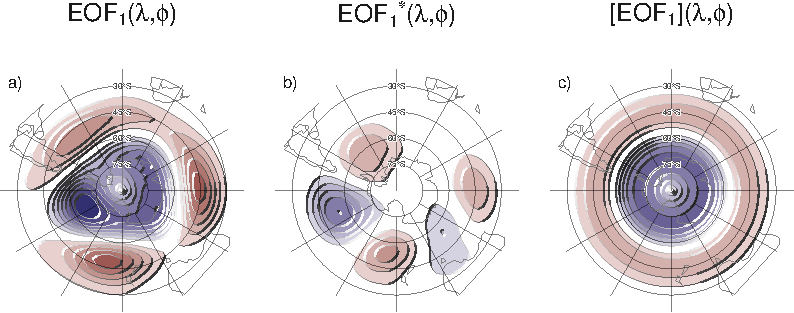
\includegraphics{method-1} \caption[Spatial patterns of the first EOF of 700 hPa geopotential height]{Spatial patterns of the first EOF of 700 hPa geopotential height. Full field (left), zonally asymmetric component (middle) and zonally symmetric component (right). Arbitrary units.}\label{fig:method}
\end{figure*}

\subsubsection{Data}

We used monthly geopotential height at 2.5 longitude by 2.5 latitude
resolution from ERA5 \citep{hersbach2020} for the period 1979 to 2018.

Monthly temperature NOAA Global Surface Temperature (NOAAGlobalTemp) 5.0
degree latitude x 5.0 degree longitude global grid
\citep{vose2012, smith2008}. The same analysis was carried out using
CRUTEM4 \citep{osborn2014} (not shown).

We used monthly precipitation data from CPC Merged Analysis of
Precipitation \citep{xie1997} 2.5 degree latitude x 2.5 degree
longitude. CPCC: {[}schneider2015{]} \#FIXME

\subsubsection{Significance}

We adjusted p-values for False Detection Rate following
\citet{wilks2016}.

\section{Results}

\subsection{Temporal evolution}

\begin{figure*}
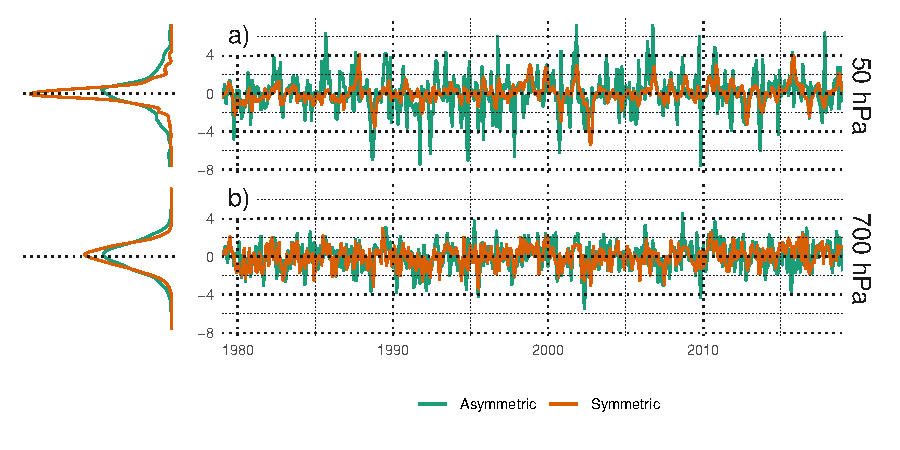
\includegraphics{asymsam-timeseries-1} \caption[Time series for the asymmetric SAM and symmetric SAM and density estimates]{Time series for the asymmetric SAM and symmetric SAM and density estimates.}\label{fig:asymsam-timeseries}
\end{figure*}

Figure \ref{fig:asymsam-timeseries} shows the resulting Asymmetric and
Symmetric time series corresponding to 700 and 50hPa. \#FIXME

At first glance the series can be distinguished by their distributions.
Whereas the tropospheric incides are aproximately normally distributed,
the stratospheric indices are more long-tailed; that is, extreme values
(both negative and positive) abound. The Asymmetric series have both
more variability in the higher frequencies than the Symmetric series.

The stratospheric Symmetric SAM varies strongly witha two-year period,
which can be seen using spectral methods (Figure A3) or in the
autocorrelation structure (Figure A4). There is a local peak at 2 years
in the periodigram of the tropospheric Symmetric SAM also, although it's
not statistically significant. In the troposphere the most significant
peak of variability is found in the Asymmetric index at around 3.6
months.

From Figure \ref{fig:asymsam-timeseries} we can see that the Asymemtric
and Symmetric time series appear to be correlated. Moreover, looking at
the extremes in the stratosphere, the Symmetric serie appears to lag the
Asymmetric series (see, for example, the positive events on late 1987
marked with a circle). We show these correlations, across all the levels
of the reanalysis and for zero and -1 lag (Asymmetric index leading the
Symmetric index), in Figure \ref{fig:cor-lev}.

\begin{figure}
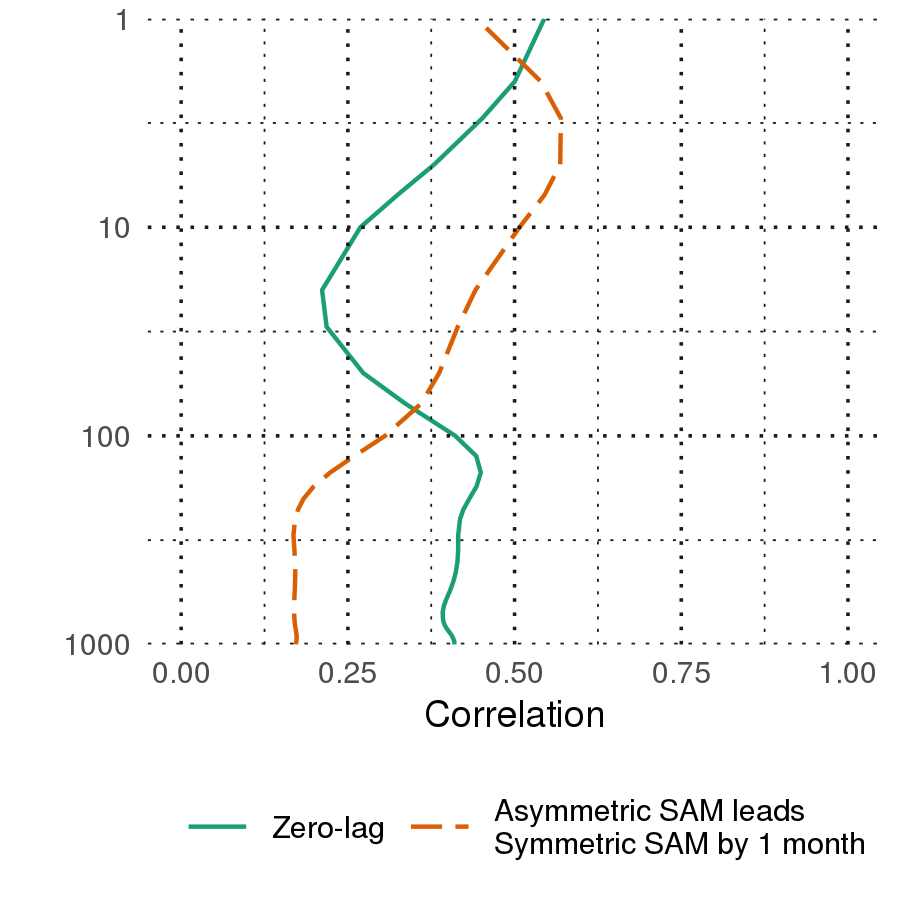
\includegraphics{cor-lev-1} \caption[Correlation between the Symmetric and Asymmetric SAM at each level for lag zero and lag -1 (Asymmetric leads Symmetric)]{Correlation between the Symmetric and Asymmetric SAM at each level for lag zero and lag -1 (Asymmetric leads Symmetric).}\label{fig:cor-lev}
\end{figure}

Zero-lag correlations between the Asymmetric and Symmetric series are
relatively constant throught the troposphere, fluctiating between 0.39
and 0.45. One-month-lag correlations are similarly constant but
significantly reduced, hovering around 0.17. In the stratosphere,
zero-lag correlations drop to a minimum of 0.21 at 20 hPa and then it
increases again monotonically with height up to the uppermost level of
the reanalysis. At the same time, one-month-lag correlations increase
with height.

\begin{figure*}
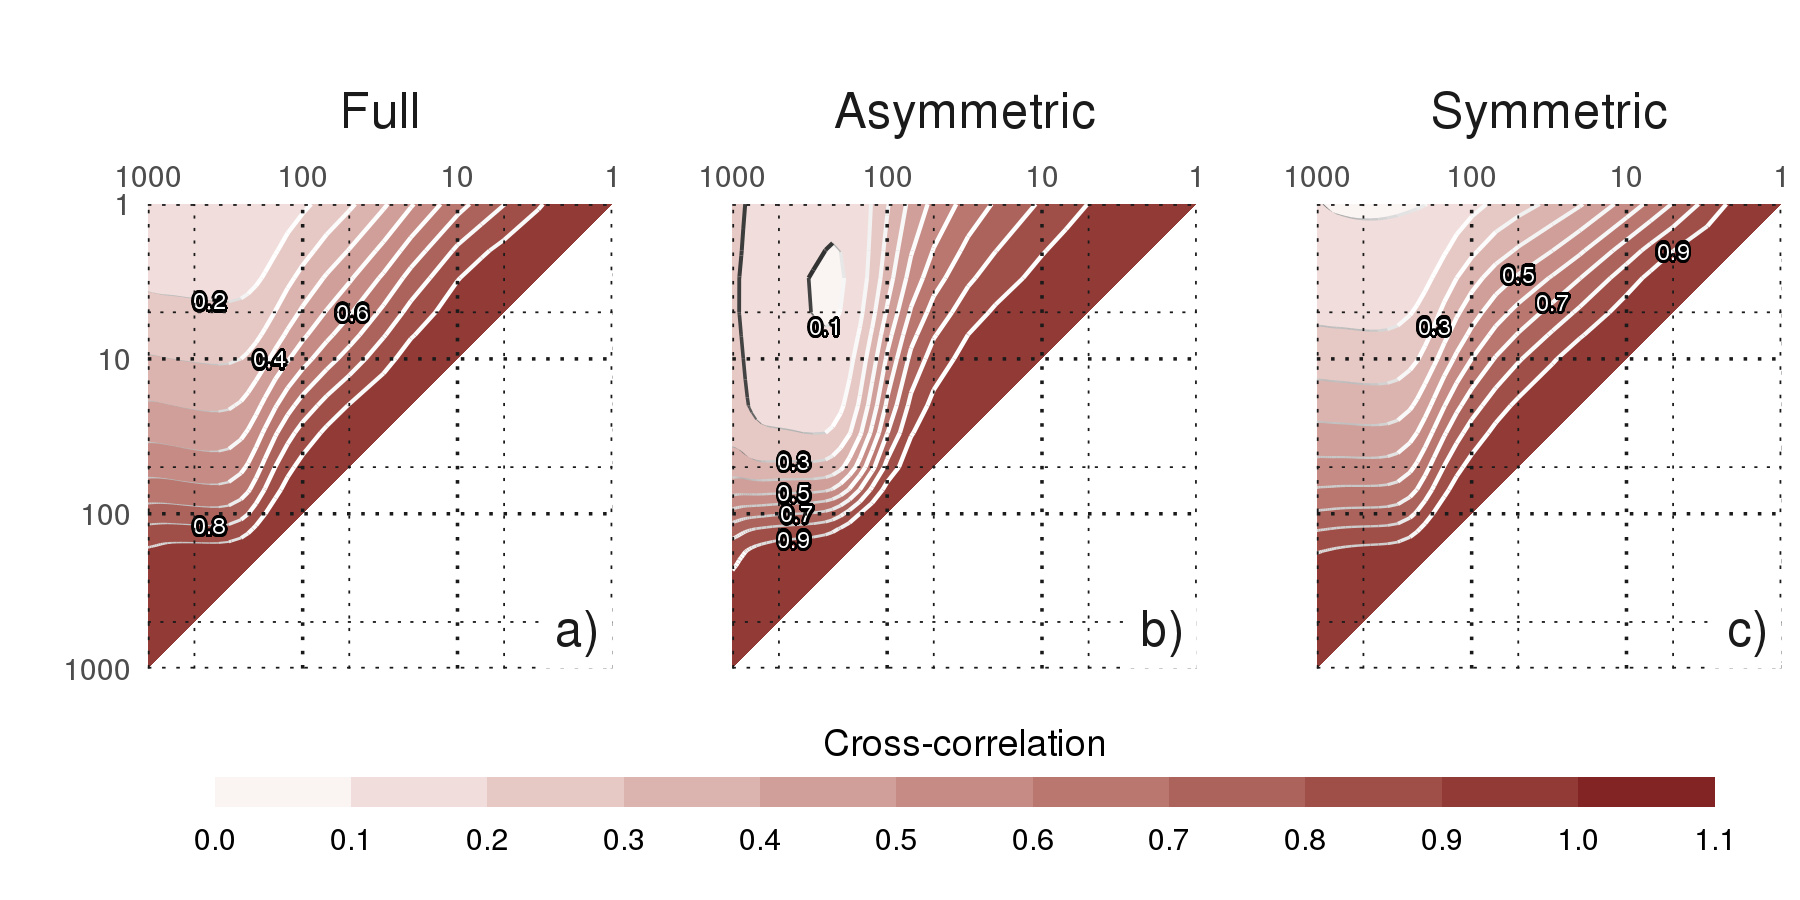
\includegraphics{cross-correlation-1} \caption[Cross correlation between levels of the Full, Asymmetric and Symmetric SAM]{Cross correlation between levels of the Full, Asymmetric and Symmetric SAM.}\label{fig:cross-correlation}
\end{figure*}

Figure \ref{fig:cross-correlation}a) shows (zero-lag) cross-correlation
across levels for the Full, Symmetric and Asymmetric SAM indices. For
the Full SAM (panel a), high values below 100 hPa reflect the vertical
(zero-lag) coherency throughout the troposfere. Above 100 hPa
correlation between levels falls off more rapidly, indicating less
coherent (zero-lag) variability. Still there is a non negligible
correlation between the troposphere and the lower-to-middle
stratosphere. Examining panels b and c, we see that the Asymemtric and
Symmetric SAM share the same high level of coherency in the troposphere
but they differ in their stratospheric behaviour. As evidenced by the
wider dark red areas near the diagonal in Figure
\ref{fig:cross-correlation}b) vs.~Figure \ref{fig:cross-correlation}c),
stratospheric coherency is stronger for the Asymmetric SAM than the
Symemtric SAM. The stratospheric Symmetric SAM seems to connect more
strongly to the trosposphere than the Asymmetric SAM; this can be seen
by the lower correlation values in the top right left of Figure
\ref{fig:cross-correlation}b) in comparison with Figure
\ref{fig:cross-correlation}c).

\begin{figure*}
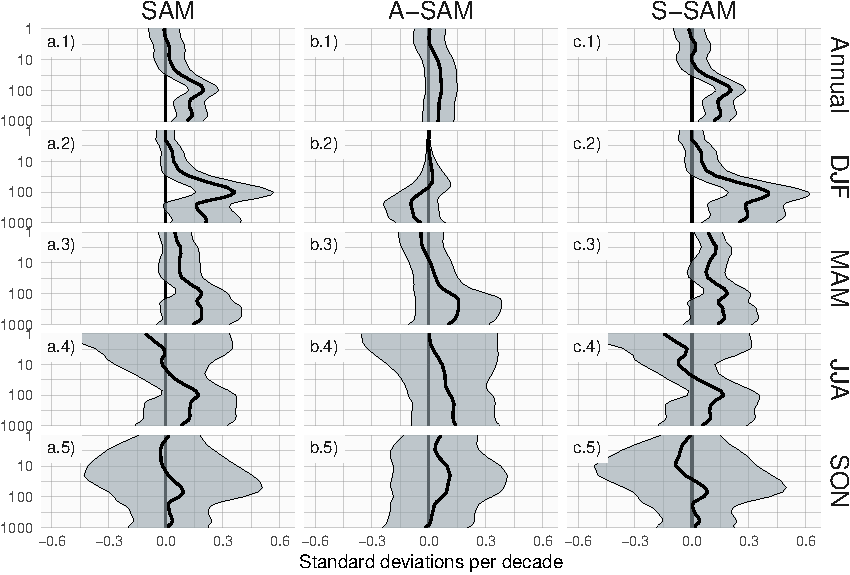
\includegraphics{trends-1} \caption[Decadal normalised trends for each index at each level for annual (row a) and seasonal values (rows b-e) for the period 1979-2018]{Decadal normalised trends for each index at each level for annual (row a) and seasonal values (rows b-e) for the period 1979-2018. Shading indicates the 95\% confidence interval.}\label{fig:trends}
\end{figure*}

Figure \ref{fig:trends} shows normalised decadal trends for each index
for the whole period 1979-2918 along with the 95\% confidence interval
in shading for the whole year (row a) and separed by trimesters (rows b
through e). As documented by \#FIXME (e.g. \citet{fogt2020}), there is a
statistically significant increase towards more positive SAM (panel
a.1), which is XX only in Summer and Autumn (panels b.1 and c.1). We
observe these increases mainly in the troposphere, reaching their
maximum at at 100 hPa in Summer. By separating the SAM signal in its
Asymmetric and Symmetric parts, we can not only see that these trends
are almost entirely due to the Symmetric component (columns 2
vs.~columns 3), but in some cases the trends become more clear. In
Summer, the Asymmetric SAM has a statistically non significant negative
trend in the middle troposphere that obscures the signal; as a result,
trends computed using only the Symmetric component are more clear
(compare the shading region in panel b.1 and b.3). In Autumn, using the
Symmetric SAM reveals a statistically significant positive trend in the
stratosphere that is not significant using the Full index.

We stress that these are only linear trends during the whole period and
the absence of a statistically significant signal should not be taken as
evidence of no sistematic change. In particular, going back to Figure
\ref{fig:asymsam-timeseries}, we can see an evident change in the
stratospheric Asymemtric component (red line in panel a) between the
90's, when we see a dominance of extreme negative values, and the 00's,
when we see the inverse. This change is restricted to the Winter months:
the linear trend for JJA starting in 1990 for the Asymmetric component
at 50hPa is \(0.37 \pm 0.22\).

Figure \ref{fig:r-squared-trend} shows decadal trends for the explained
variance of each index. There is no evidencie of a significant trend in
the stratosphere. In the troposphere, there is a positive trend for the
Asymmetric SAM and no significant trend for the Symmetric SAM. This
suggest that the SAM has become more asymmetric in the period from 1979
to 2018. The change is slight, though; of the order of 1\% icreased
explained variance per decade.

\begin{figure}
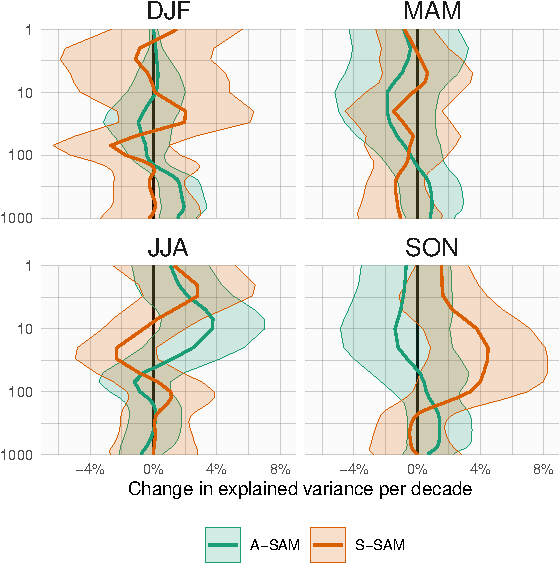
\includegraphics{r-squared-trend-1} \caption[Decadal trends for explained variance of each index at each level for the period 1979-2018]{Decadal trends for explained variance of each index at each level for the period 1979-2018. Shading indicates the 95\% confidence interval.}\label{fig:r-squared-trend}
\end{figure}

\subsection{Spatial patterns}

To undertand the spatial patterns associated with both indeces, we
regressed monthly geopotential anomalies into both indeces using
multiple regression

\begin{figure*}
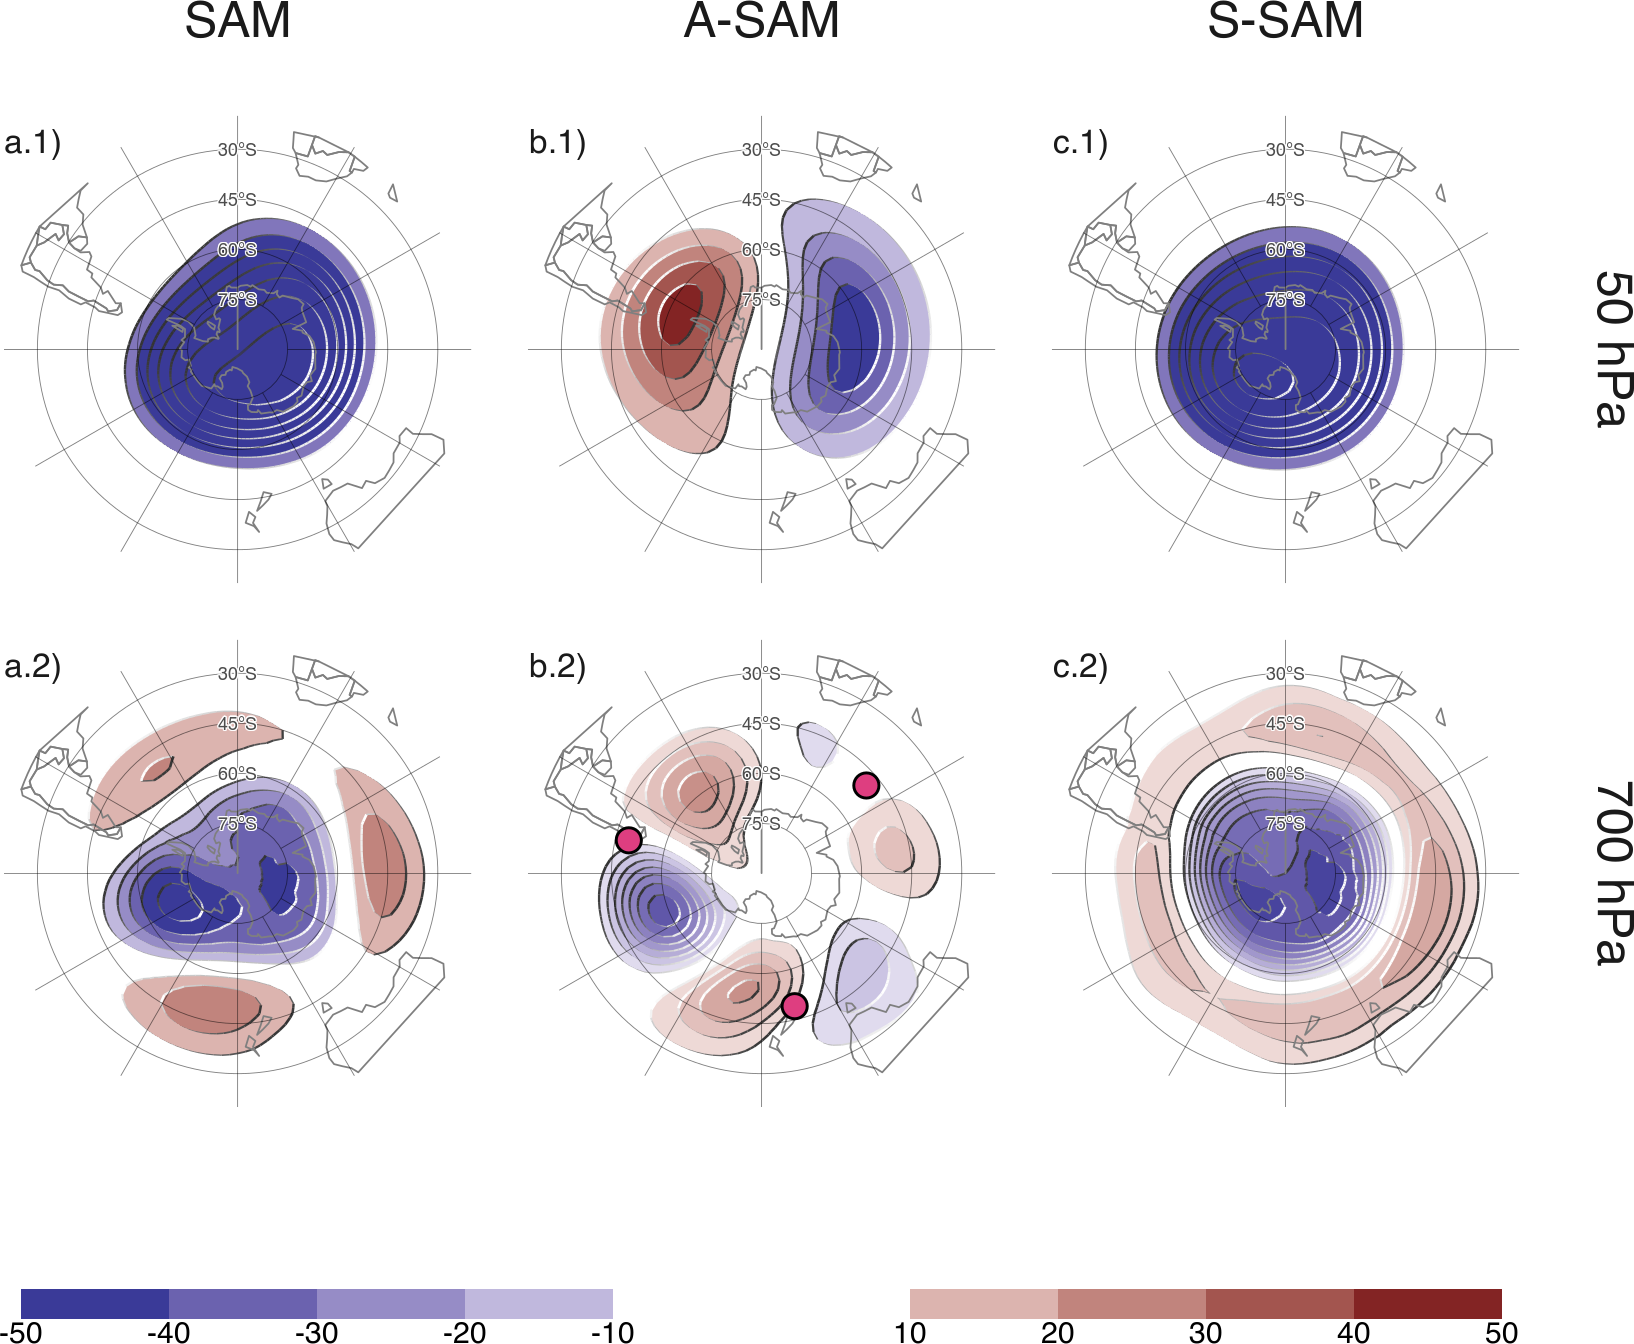
\includegraphics{2d-regr-1} \caption[Regression patterns of geopotential height at 30, 300 and 700 hPa with the Full, Asymmetric and Symmetric SAM]{Regression patterns of geopotential height at 30, 300 and 700 hPa with the Full, Asymmetric and Symmetric SAM. The regression patterns for Asymmetric and Symmetric SAM are the result of one multiple regression using both indices, not of two simple regressions involving each index by itsef.}\label{fig:2d-regr}
\end{figure*}

Figure \ref{fig:2d-regr} shows the spatial year-long regression \#FIXME.
Column a are regressinos using the Full SAM, while columns 2 and 3 are
regression coefficients computed in a multiple regression of
geopotential height on the Asymmetric and Symmetric indices at the same
time. Thus, they are to be interpreted as the patterns associated with
each index, controling for the (linear) effect of the other. (Figure A6
\#FIXME illustrates the difference between computing two simple
regressions and one multiple regression.)

In the stratosphere, the spatial pattern associated with the Full SAM is
more clearly dominated by a zonally symmetric, monopolar structure
(panel a.1) which is, however, not perfectly centered in the south pole.
The monopole obtained by multiple regression with the Asymmetric and
Symmetric SAM (panel a.3) is much more symmetric and the shift from
total symmetry is captured by the regression pattern of the Asymmetric
SAM as a wave-1 with maximum anomalies above the Belinghausen Sea on the
Western Hemisphere and and Davids Sea in the Eastern Hemisphere (panel
a.2).

In the troposphere, panel b.1 shows the well known zonally symmetrical
annular mode \emph{contaminated} with zonal asymmetries in the form of a
wave-3. The regression using the Asymmetric and Symmetric SAM indices
successfully disentangle both structures. The Asymmetric component gives
rise to a cleaner zonal wave (panel b.2) and the Symemtric component is
assosiated with an trully annular mode, almost devoid of zonal
asymmetries (panel b.3). note that the wave-3 pattern observed in panel
b.2 is rotated by half a wavelength from the average position of the
mean wave-3 pattern and asociated with \citet{raphael2004}'s ZW3 index
(see Figure 1 from that paper). \#FIXME (agregar algo más?)

\begin{figure}
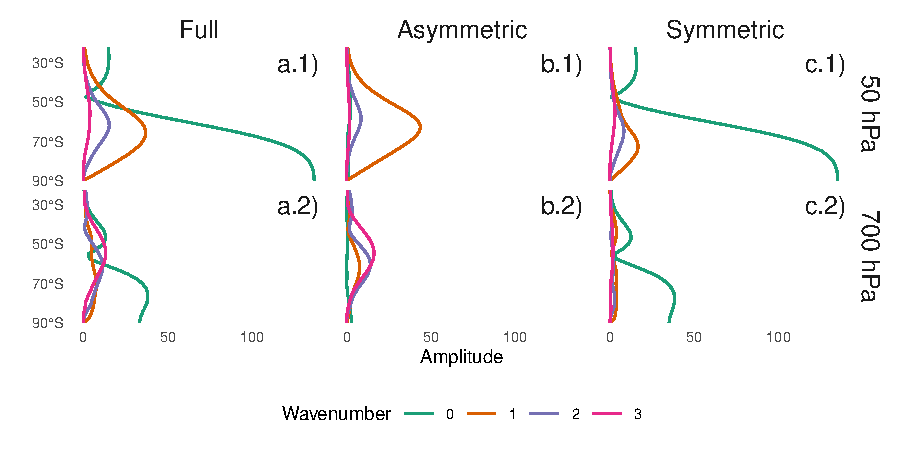
\includegraphics{wave-amplitude-1} \caption[Planteray wave amplitude for the regression patterns at 50 and 700 hPa]{Planteray wave amplitude for the regression patterns at 50 and 700 hPa. Note the varying x axis.}\label{fig:wave-amplitude}
\end{figure}

The amplitude of each zonal wave number at each latitude at 50 hPa and
700 hPa is shown in Figure \ref{fig:wave-amplitude}, where wave number
zero represents the amplitude of the zonal mean. Comparing between rows,
this Figure quantifies the relatively clean separation between the
zonally symmetric and zonally asymmetric structures, as its evident how
the mixture of waves of the Full field (column a) is very similar to the
sum of the waves of the Asymmetric and Symmetric field (columns b and c,
respectively). Column b of Figure \ref{fig:wave-amplitude} shows that
the Asymmetric SAM is overwhelmingly dominated by wave 1 in the
stratosphere (panel b.1), while in the troposphere it is composed of
zonal waves 3 to 1 in decreasing level of importance (panel b.2).

\begin{figure}
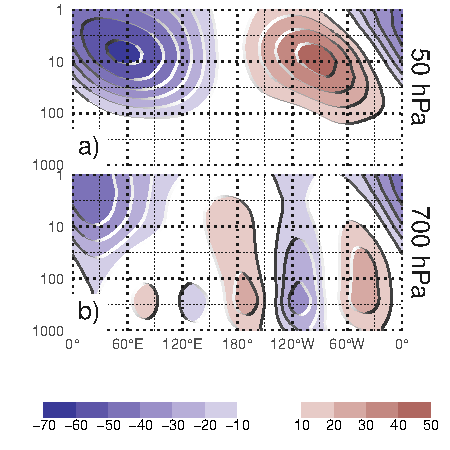
\includegraphics{vertical-regression-1} \caption[Asymmetric coefficient of the multiple regression of mean monthly geopotential height anomalies between 65 and 40 South]{Asymmetric coefficient of the multiple regression of mean monthly geopotential height anomalies between 65 and 40 South. (\#FIXME this caption needs some love)}\label{fig:vertical-regression}
\end{figure}

To analyse the vertical structure of the geopotential anomalies
asociated with the asymetric SAM index, we show a vertical cross section
of regressions of mean geopotential height between 65ªS and 40ªS for the
50 hPa Asymmetric SAM index (panel a) and for the 700 hPa Asymmetric SAM
index (panel b) (Figure \ref{fig:vertical-regression}).

The geopotential anomalies associated with the stratospheric SAM (panel
a) are clearly constrained to the stratosphere, which underscores the
disconnect between the stratospheric and tropospheric symetric SAM. The
vertical structure this signal tilts about 60ª to the West between 100
hPa and 1 hPa, suggesting baroclinic processes and polarward transport
of heat (\#FIXME is this ok?). Interestingly, the signal in the
stratosphere maximises near 10 hPa despite using the 50 hPa index for
the regression.

The tropospheric asymmetric SAM has significant signals that extend
upwards the uppermost levels of the reanalysis. In the troposphere, the
wave-3 structure is equivalent barotropic with maximum amplitude at
roughly 250 hPa. \#FIXME moaaaaar.

Interestingly, the structures shown in Figure
\ref{fig:vertical-regression} are surprisignly robust to the choice of
index level. For any stratospheric (above 100 hPa) index, the resulting
anomalies are very similar to the wave-1 structure with maximum near 10
hPa in panel a. Conversely, for any tropospheric (below 100 hPa) index,
the result is very similar to panel b. The pattern cross-correlation
between levels of each segment of the atmosphere is greater than 0.9
(Figure A8). The patterns mainly change in amplitude. The tropospheric
pattern is maximised by the 300 hPa Asymmetric SAM index and the
stratospheric pattern increased monotonically with height.

The wave-3 pattern from Figure \ref{fig:2d-regr} panel b.2 is very
similar to the teleconnection pattern associated with the ENSO. Indeed,
\citet{fogt2011} showed that there is a significant relationship between
the SAM and the ENSO. The correlation between the full SAM and the ENSO
as measured by the Multivariate Enso Index \citep{wolter2011} is -0.19.
This relationship is captured entirely the Asymmetric SAM, as this index
has a partial correlation of -0.27 with the MEI, whereas the Symmetric
SAM has null partial correlation with the MEI.

\subsection{Impacts}

\subsubsection{Temperature}

\begin{figure*}
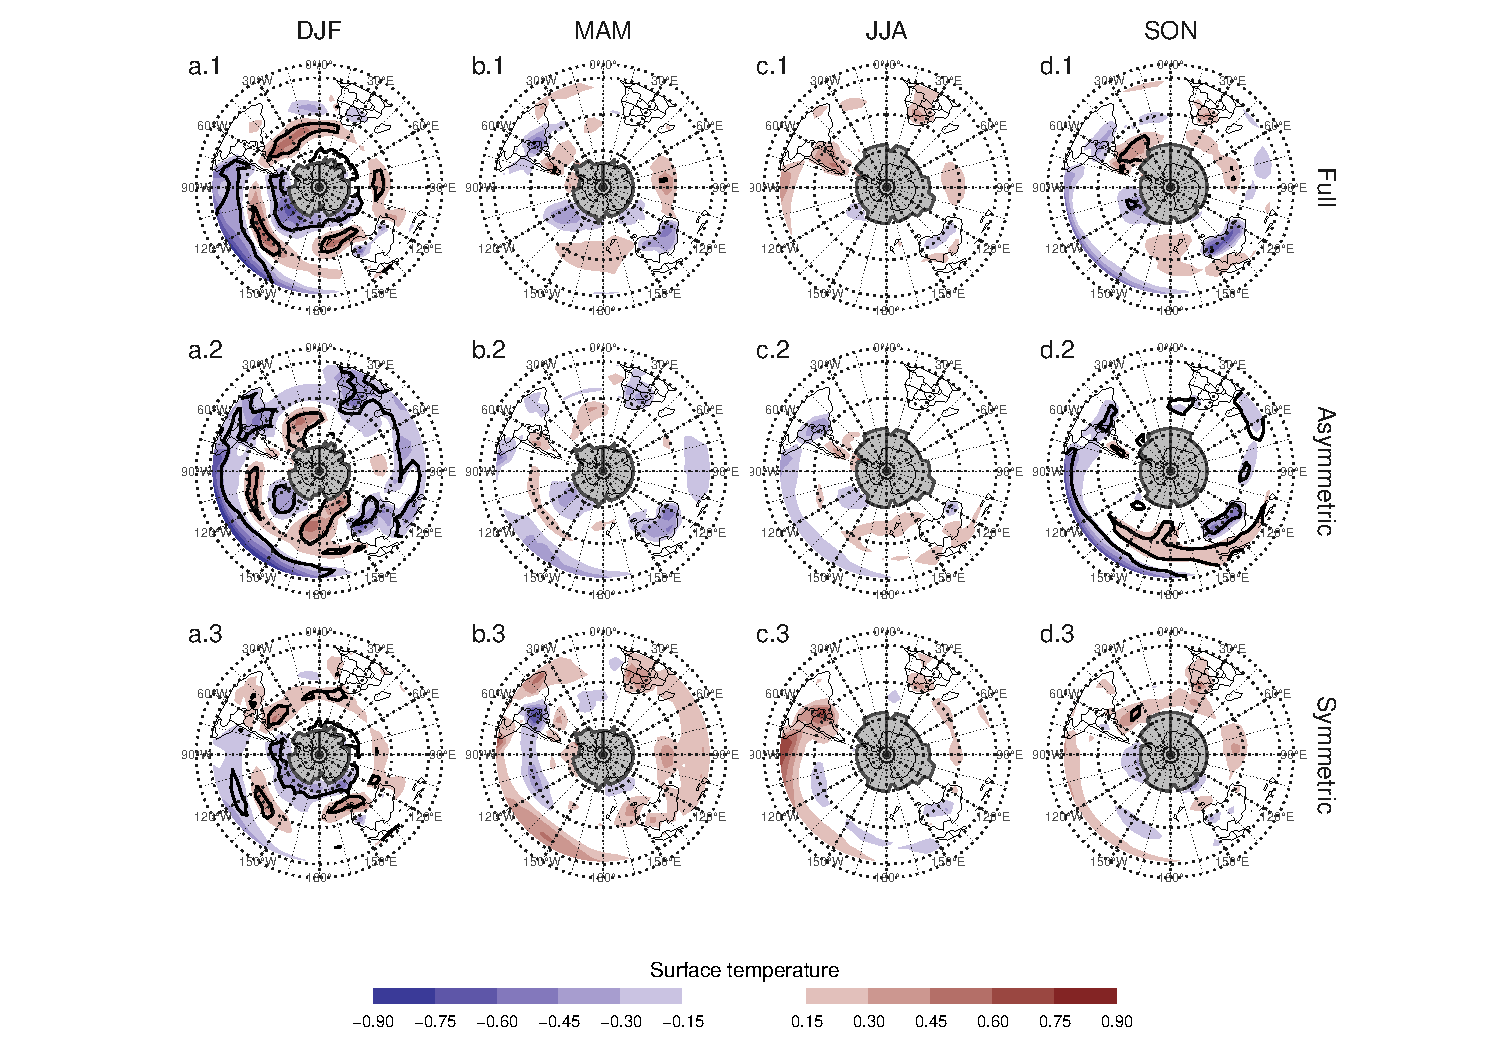
\includegraphics{regr-air-season-1} \caption[Regression pattern of surface temperature with Asymmetric and Symmetric SAM]{Regression pattern of surface temperature with Asymmetric and Symmetric SAM. P-values smaller than 0.05 (controlling for Flase Detection Rate) as hatched areas. Gray areas have more than 15\% of missing data.}\label{fig:regr-air-season}
\end{figure*}

Figure \ref{fig:regr-air-season} shows regression coefficients of each
index at 700 hPa with surface temperature for each trimester. It is
evident that the Asymmetric and Symmetric SAM indices are associated
with overall distinct temperature patterns which can be obscured when
using the Full SAM index. The Symmetric SAM signal is weaker than the
Asymmetric SAM, as evidenced by the relatively smaller and les
sstatistically significant regression coefficients in row 3 of Figure
\ref{fig:regr-air-season} compared with row 2.

In DJF (column a), the strong negative signal in the tropical Pacific in
panel a.1 is mostly associated with the Asymmetric component (panel
a.2), as is it largely absent in the Symmetric component (panel a.3).
Furthermore, the Asymmetric SAM is also asociated with low temperature
anomalies in the Indian ocean, but this signal is obscured by the
Symmetric variability and thus lost in the Full SAM. Over the
continents, the Asymmetric SAM is assoiated with negative temperature
anomalies which, again, mostly disappear in the Full SAM regression.

The patterns seen in MAM and JJA (columns b and c) are not robustly
significant in the sense that there are no areas with p-values below
0.05 when controlling for FDR following \citet{wilks2016}. Nevertheless,
it is interesting to note that in both trimesters, the sign of the
regression is consistently flipped between the Asymmetric and Symmetric
regressions. In South America, for example, the Asymmetric SAM is
associated with positive temperature anomalies in MAM and negative
temperature anomales in JJA, while the oposite is the case for the
Symemtric SAM.

Finally, in SON (column d), there is no significant temperature signal
associated with the Symmetric SAM (panel d.3), while the Asymmetric SAM
shows a relatively robust signal in the equatorial Pacitic, Australia,
and even Southeast South America. This strong signals are reduced in
intensity in panel a.3.

\subsubsection{Precipitation}

Regression of the SAM indicies with seasonal mean precipitation are
shown Figures \ref{fig:pp-regr-oceania} and \ref{fig:pp-regr-america}
for Australia and New Zealand, and South America respectively. (We
didn't detect any significant signal in South Africa.)

\begin{figure*}
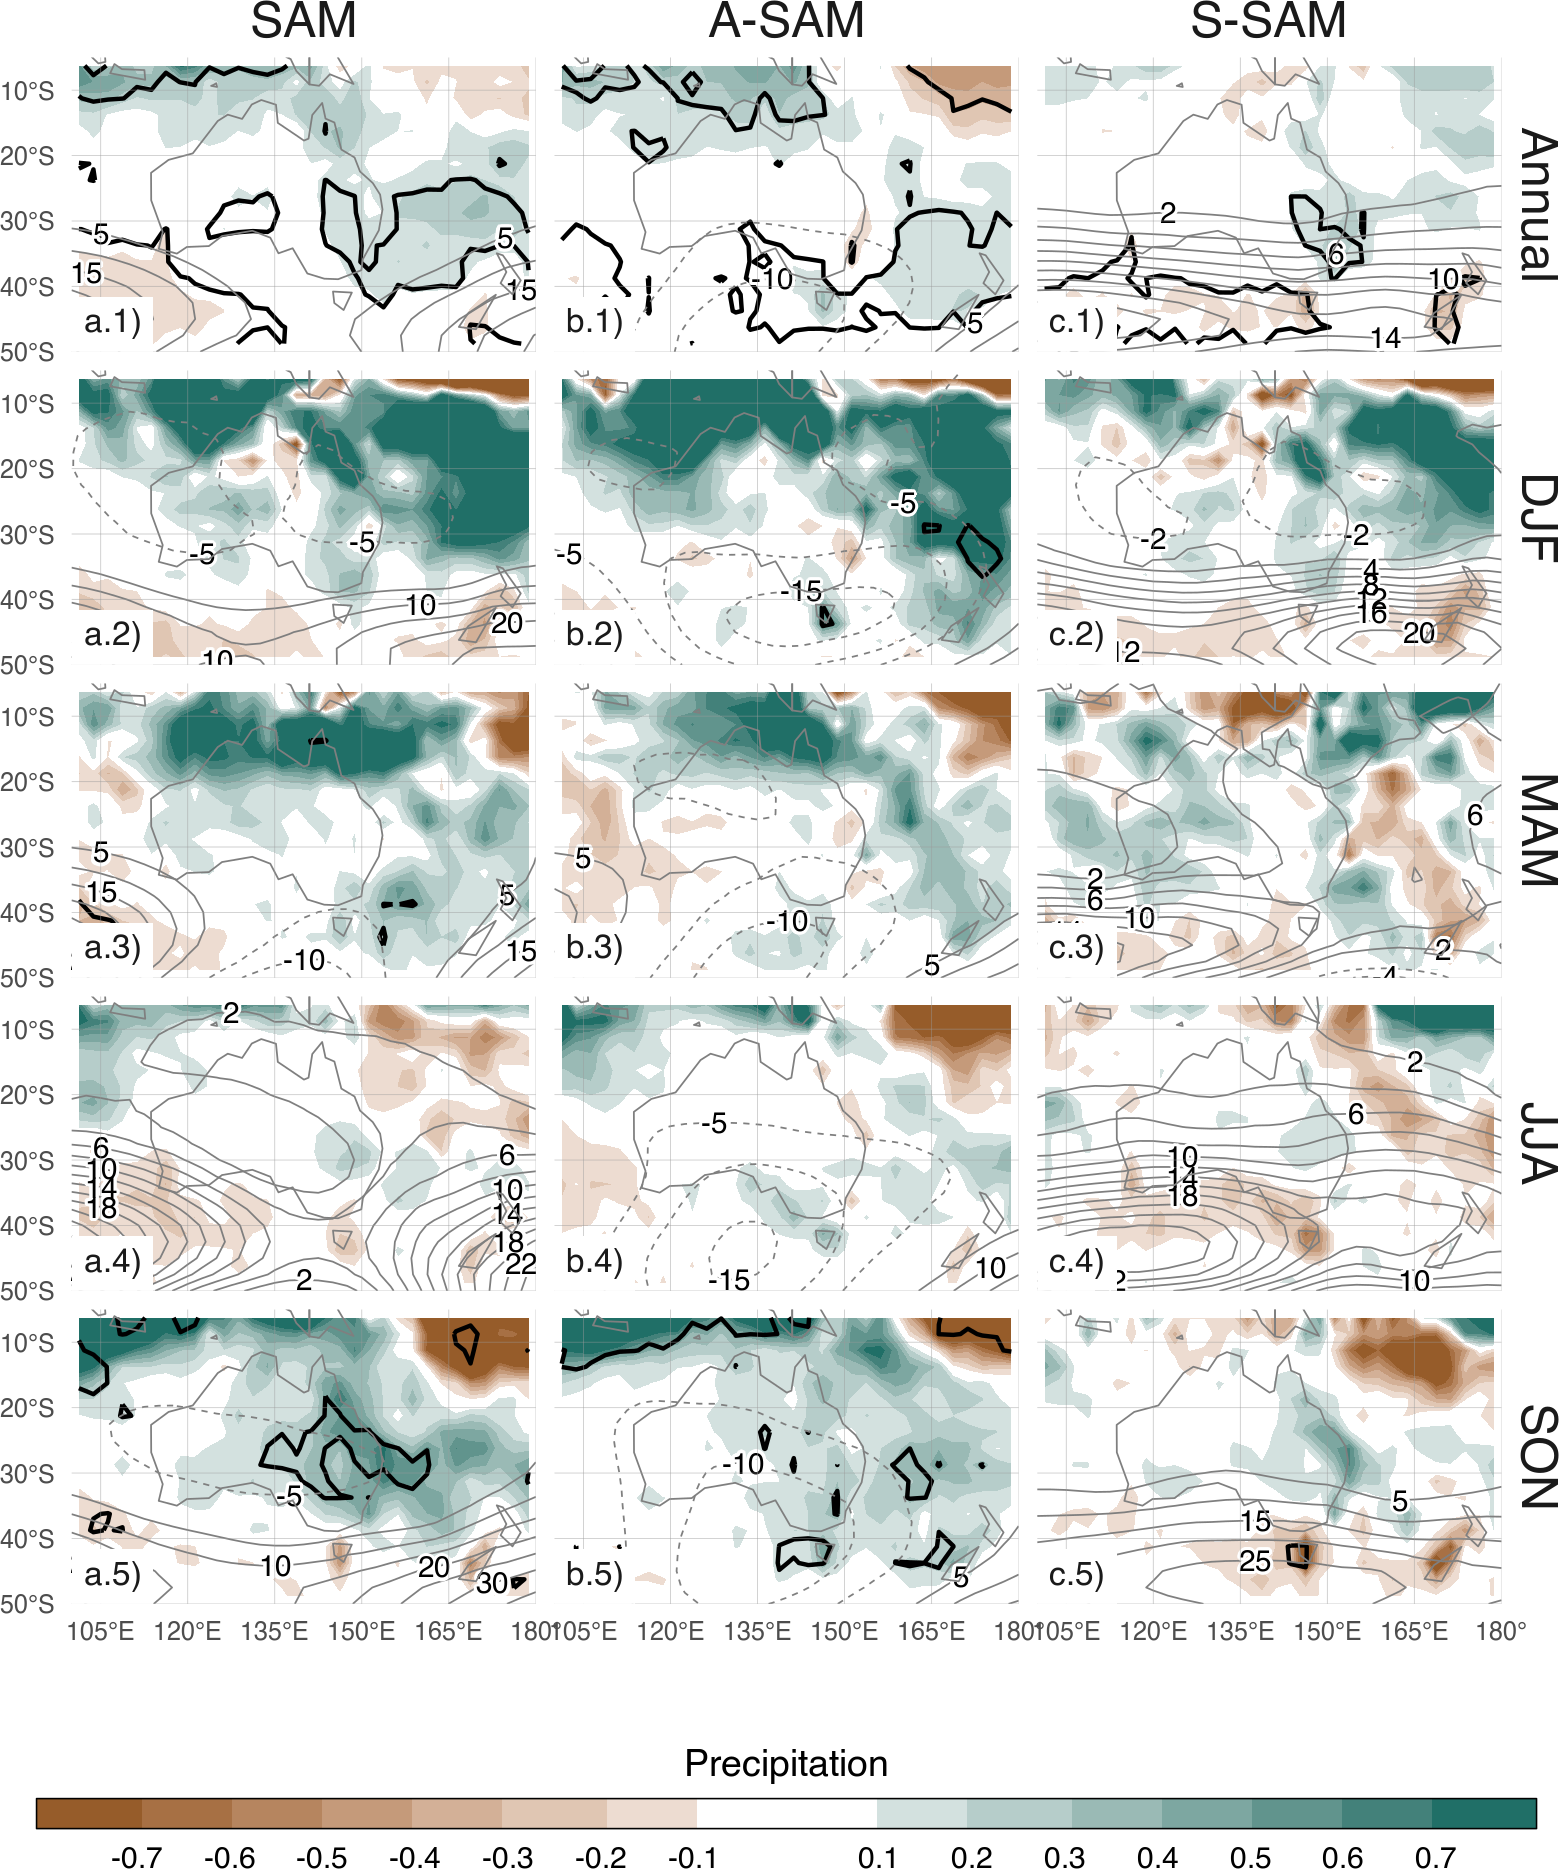
\includegraphics{pp-regr-oceania-1} \caption[Same but for oceania]{Same but for oceania}\label{fig:pp-regr-oceania}
\end{figure*}

In Australia (Figure \ref{fig:pp-regr-oceania}), the annual-level
regression shows that the Full SAM is associated with a statistically
significant increase in precipitation in the Southeastern region (panel
a.1), which reproduces the results from \citet{gillett2006}. The
separation between Asymmetric and Symmetric SAM suggest that this
increase is explained by the Symmetric SAM only in the East coast (panel
c.1), which is consistent with the increased easterly flow clearly seen
in relation with this index. The Asymmetric SAM appears related to
increased precipitation in the West coast of Southeastern Australia
(panel b.2), explained by the anomalous \emph{westerly} circulation
transporting moist air to the continent.

The seasonal-level regressions show statistically significant anomalies
only in SON, with a pattern similar to the annual-level regression
(panel a.5). Panels b.5 and c.5 don't show a clear separation between
the Asymmetric and Symmetric SAM. If anything, the positive and more
significant regression coefficients in panel b.5 vs pane c.5 would
suggest more influence of the Asymmetric than the Symmetric SAM, going
against the interpretation gathered from the annual-level regressions.
This Spring signal is broadly consistent with \citet{hendon2007}, but
whereas \citet{hendon2007} also detected a strong signal in Summer,
panel a.2 shows no statistically significant association (although the
coeffcients have the consistent sign).

\begin{figure*}
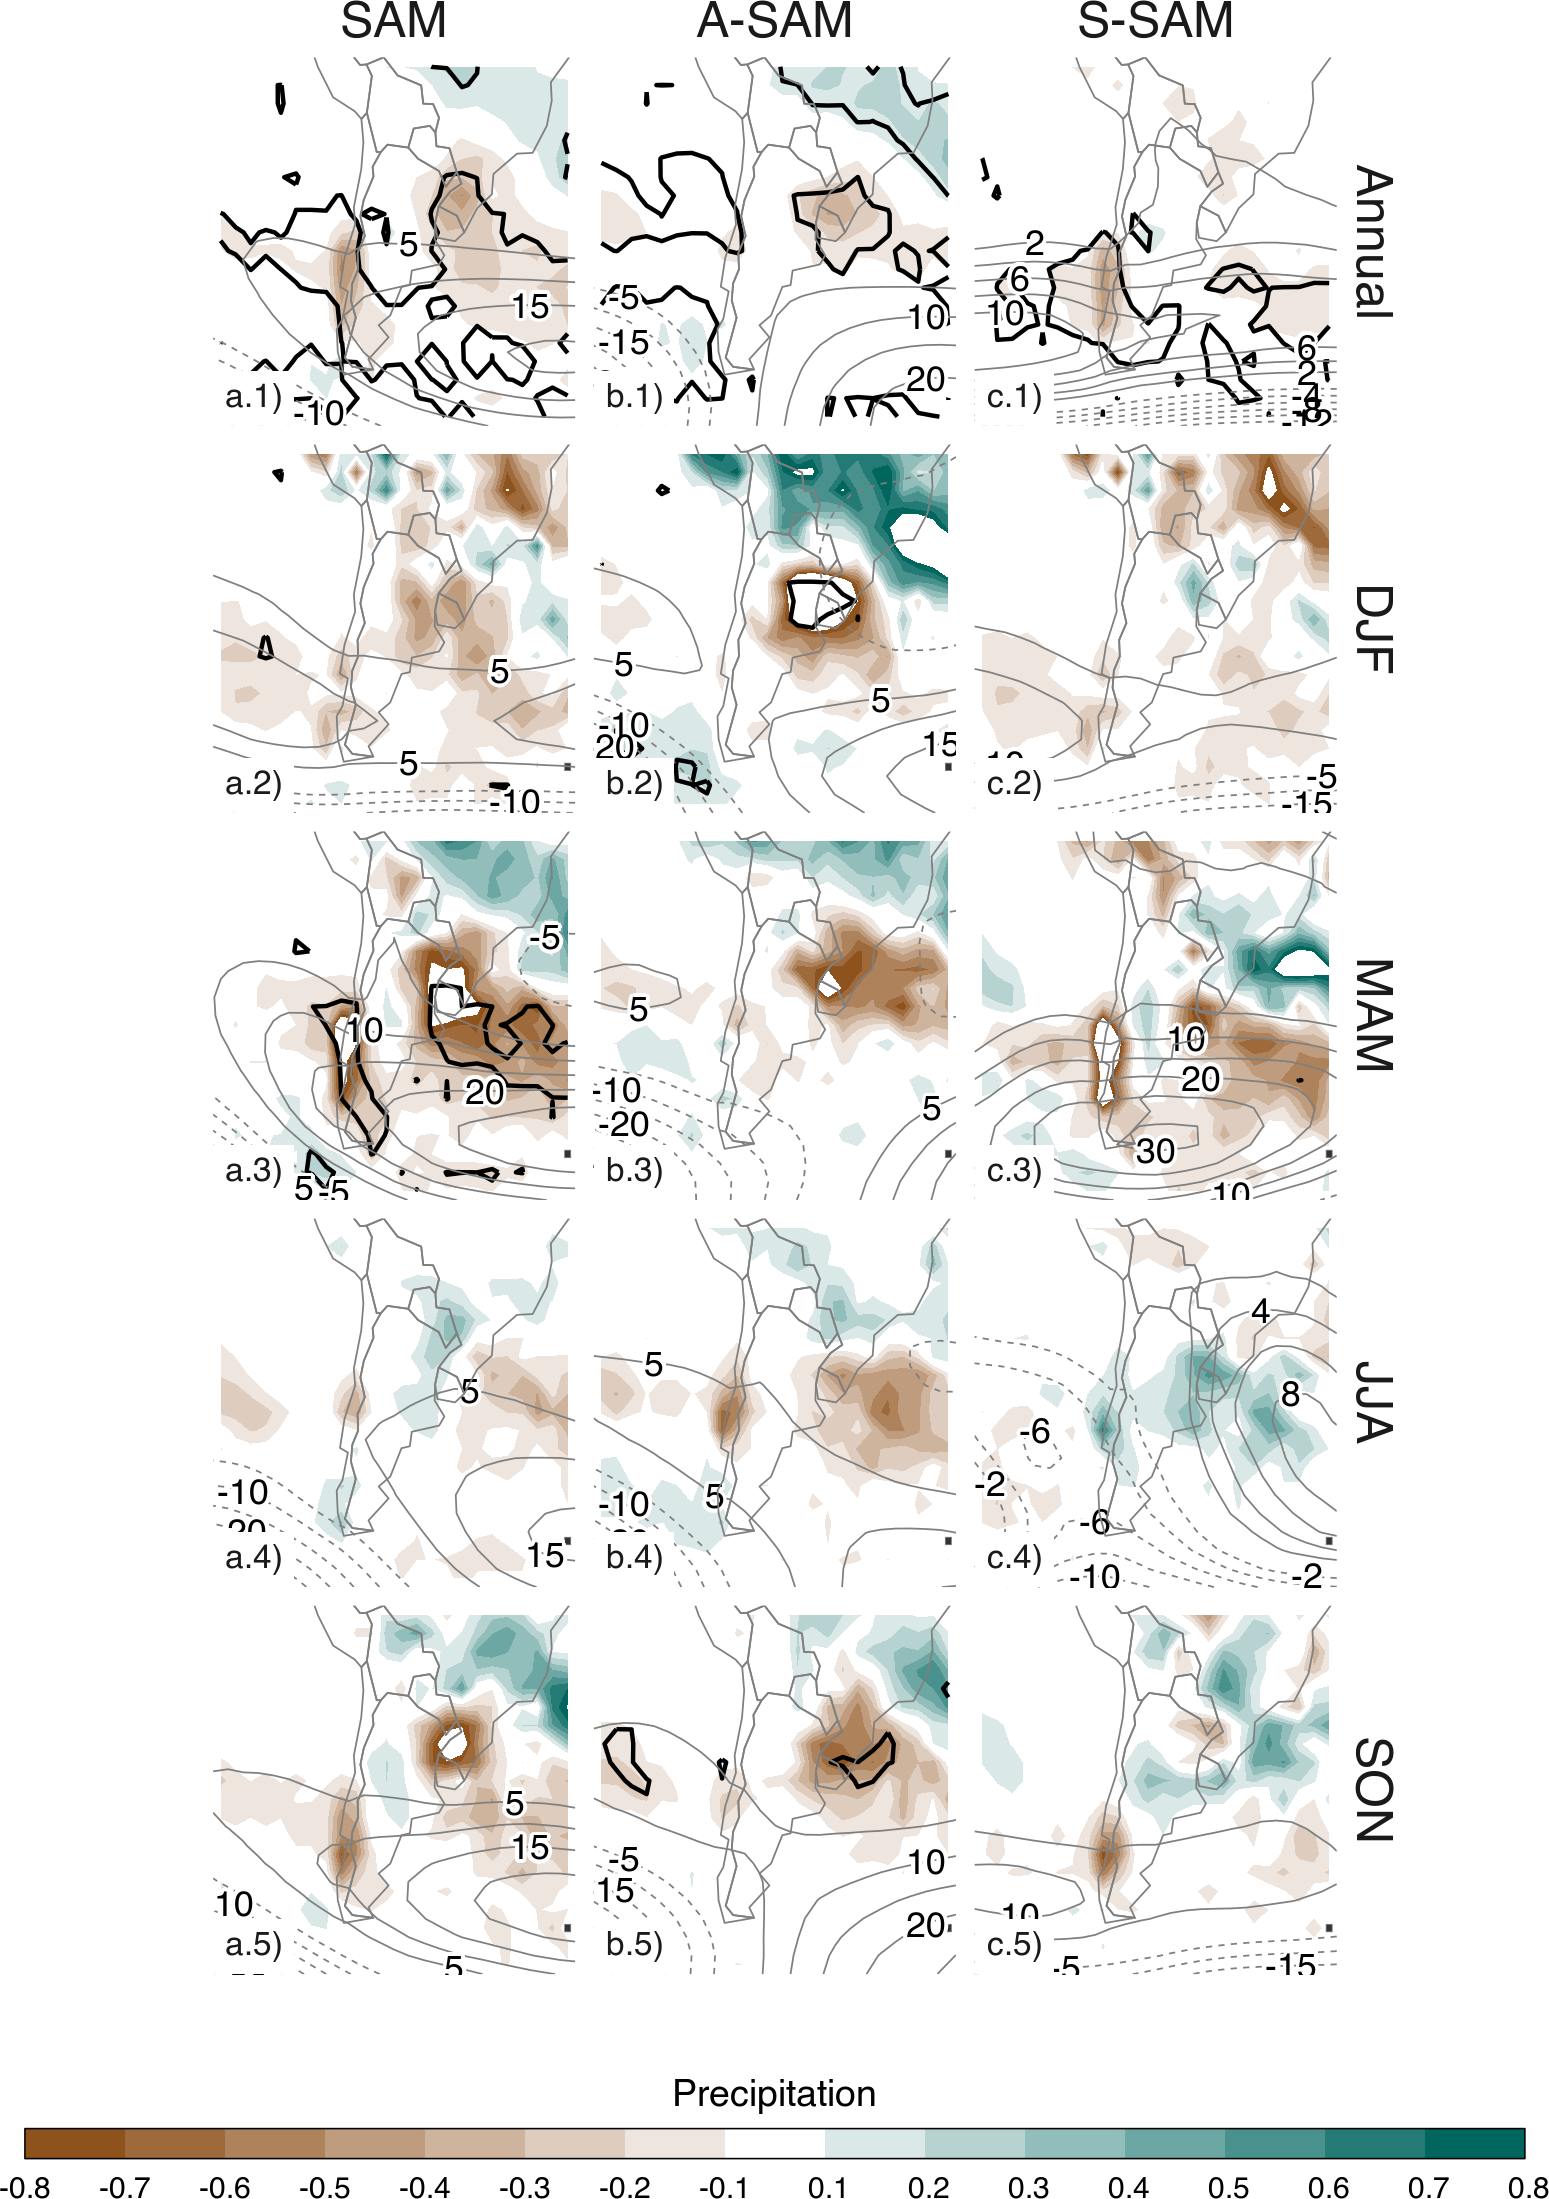
\includegraphics{pp-regr-america-1} \caption[Same but for america]{Same but for america}\label{fig:pp-regr-america}
\end{figure*}

In South America (Figure \ref{fig:pp-regr-america}), the annual-level
regression shows that the SAM is associated with statistically
significant precipitation decrease in Southeastern South America (SESA)
and Southern Chile and non-significant increase in South Brazil, near
the South Atlantic Convergence Zone (SACZ) (panel a.1).

Panels b.1 and c.1 show a remarkably clean separation between the
Asymmeric SAM --associated with the Southeastern South American and
Southern Brazilian signals-- and the Symmetric SAM --associated with the
signal in Southern Chile. This separation is consistent with the
mechanisms responsible for these effects. In Southern Chile, the reduced
westerly flow reduce moisture transport from the Pacific Ocean (cita??
\#FIXME).

In Southeastern South America, anomalous meridional winds lead to less
precipitation by inhibiting moisture convergence from the South American
Low Level Jet \citep{silvestri2009}. The increased precipiation in the
South Atlantic Convergence Zone, on the other hand, appears to be
related to modulation of the anomalous SAM circulation in SACZ events
which lead to more frequent and intense SACZ events during positive SAM
\citep{rosso2018}.

There is a small area of increased precipitation with SAM near central
Argentina which is also present in the station-based analysis by
\citet{gillett2006} and that is explained by the Asymmmetric SAM.

Except during Winter, the seasonal-level regression all show these
similar patterns although not as cleanly and only in some cases
statistically significant.

\subsubsection{Sea ice}

\begin{figure*}
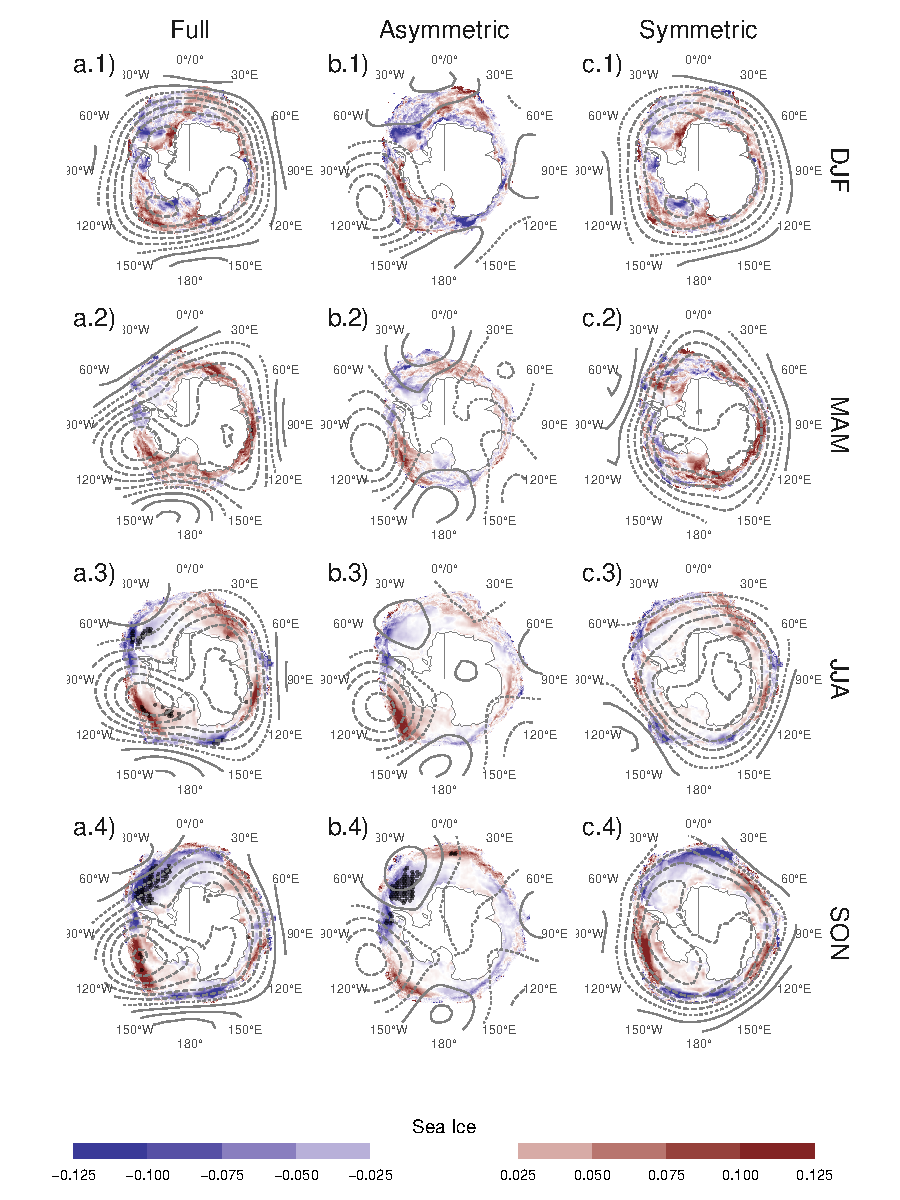
\includegraphics{regr-ice-1} \caption[Seasonal regression of SAM indices with sea ice concentration]{Seasonal regression of SAM indices with sea ice concentration. \#FIXME}\label{fig:regr-ice}
\end{figure*}

Regressions between the Full SAM index and Antarctic Sea Ice
Concentrations (Figure \ref{fig:regr-ice}) show a great deal of
variability across seasons. The only statistically significant signal is
in Spring, when we observe negative concentraion anomalies in the
Northen Weddell Sea (panel a.4) explained by the Asymmetric SAM (panel
b.4). Both in Winter and in Spring the Asymmetric SAM is associated with
bigger Sea Ice Concentration anomalies in West Antarctica than East
Antarctica, with generally decreased concentration East of the Antarctic
Peninsula and increased concentration to the West, as expected from the
anomalous circulation correlated with this index. The Symmetric SAM
signal appears more evenly distributed accross the whole ice sheet.

\subsection{Conclusions}

We presented a method to systematically separate the zonally asymmetric
and zonally symmetric components of the SAM. By itself, the spatial
structure and temporal evolution of the SAM shows a strong separation
between the stratosphere SAMs. The first EOF in the stratosphere is
monopolar in nature while the first EOF in the troposphere is a proper
annular mode. Their repespective departures from the zonal mean are also
different: a zonal wave 1 dominates the stratospheric SAM, waves 3 and 2
dominate the tropospheric SAM. Furthermore, there is little temporal
correlation between the tropospheric and stratospheric time series.

The zonal asymmetric component of the SAM at each level is even more
decupled between the troposphere and the stratosphere. Their temporal
evolution shows essentialy zero correlation (Figure
\ref{fig:cross-correlation}) and the signal associated with the
stratospheric Asymmetric SAM is completely restricted to the
stratosphere (Figure \ref{fig:vertical-regression} panel a).
Geopotential height anomalies associated with the tropospheric
Asymmetric SAM, on the other hand, do extend to the stratosphere, but
those anomalies do not project strongly into the stratospheric
Asymmetric SAM.

We show that the observed positive trends towards positive SAM is
restricted to the tropospheric SAM and is explained by the Symmetric
component (Figure \textbackslash{}ref\{fig:trends{]}). However, the
degree of asymmetry appears to have increased slightly in the last 40
years, as the Asymmetric SAM explains an increasingly proportion of the
variance (Figure \ref{fig:r-squared-trend}).

In terms of impacts, we see that ..Temperature\ldots{} \#FIXME

The patterns of SAM-associated precipitation anomalies are similarly
well separated. In South America, we show that negative anomalies
observed in Chile related to the SAM are well explained by the Symmetric
compomnet, while the precipitation dipole in Southern South America and
the South Atlantic Convergence Zone is explained by the Asymmetric
component.

\subsubsection{Limitations}

Our method assumes linearity in the asymmetric component of the SAM.
That is, assumes that zonal symmetries associated with positive SAM are
oposite and equal to the ones associated with negatie SAM.
\citet{fogt2012}'s composites suggest that this might not be entirely
valid, although we argue that much of that apparent non-linearity is due
to the heterogenous nature of the selected years for constructing the
composites. Using our data (from 1979 to 2018), seasonal composites of
zonal anomalies of 700 hPa geopotential height for for SAM+ and SAM-
show pattern linear correlations greater than -0.7 for all seasons and
are visually very linear (Figure A9). Therefore, we belive that our
method is at the very least a reasonable approximation of the fenomenon.

We also asumed that the structure of the SAM zonal anomalies is stable
in all seasons. Again, this is not unreasonable, as geopotential zonal
anomalies computed by projecting the first EOF \emph{of each season} are
very similar to each other (Figure A10).

\citet{silvestri2009} showed that impacts linked to the SAM changed
rather dramatically before and after 1980. In particular, the negative
relationship with precipitation in South America (consistent with Figure
\ref{fig:pp-regr-america} panel a.1) was absent in some areas and
switched sign in other in the earlier period. The correlation between
ENSO and SAM is similarly non-stationary, also disapearing before 1973.

Seeing as both the ENSO-SAM relationship and most of the precipitation
imacts in South America are captured by the Asymmetric SAM, the results
presented here are most likely period-dependent. Therefore, is very
likely that if we were to repeat this analysis using pre-satellite data,
the resulting Asymmetric SAM would look very different.

\acknowledgments

CMAP Precipitation data provided by the NOAA/OAR/ESRL PSL, Boulder,
Colorado, USA, from their Web site at https://psl.noaa.gov/ \#FIXME

NOAA Global Surface Temperature (NOAAGlobalTemp) data provided by the
NOAA/OAR/ESRL PSL, Boulder, Colorado, USA, from their Web site at
https://psl.noaa.gov/

\bibliography{AsymSAM}

\newpage

\appendix

\appendixtitle{Extra figures}

\begin{figure}
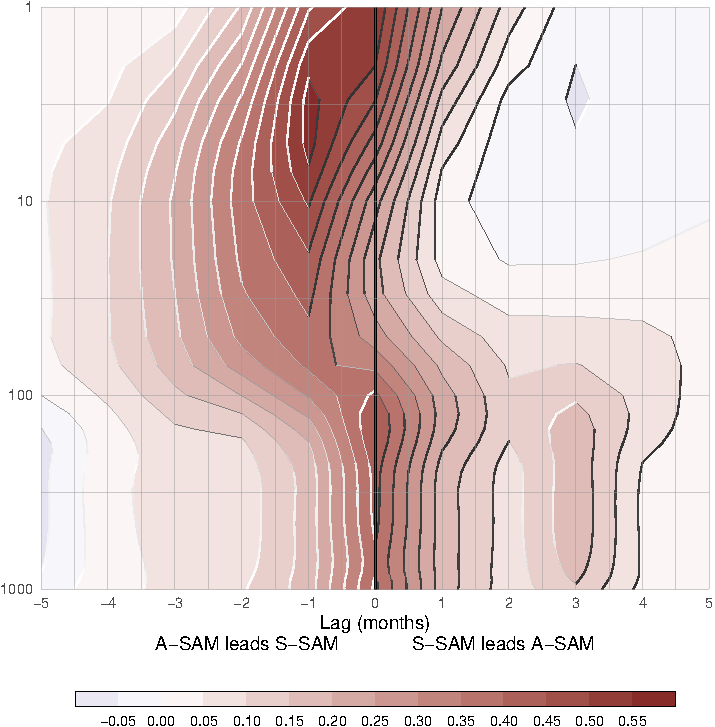
\includegraphics{A1-1} \appendcaption{A1}{Lag-correlation between Symmetric and Asymmetric SAM at each level.}\label{fig:A1}
\end{figure}

\begin{figure}
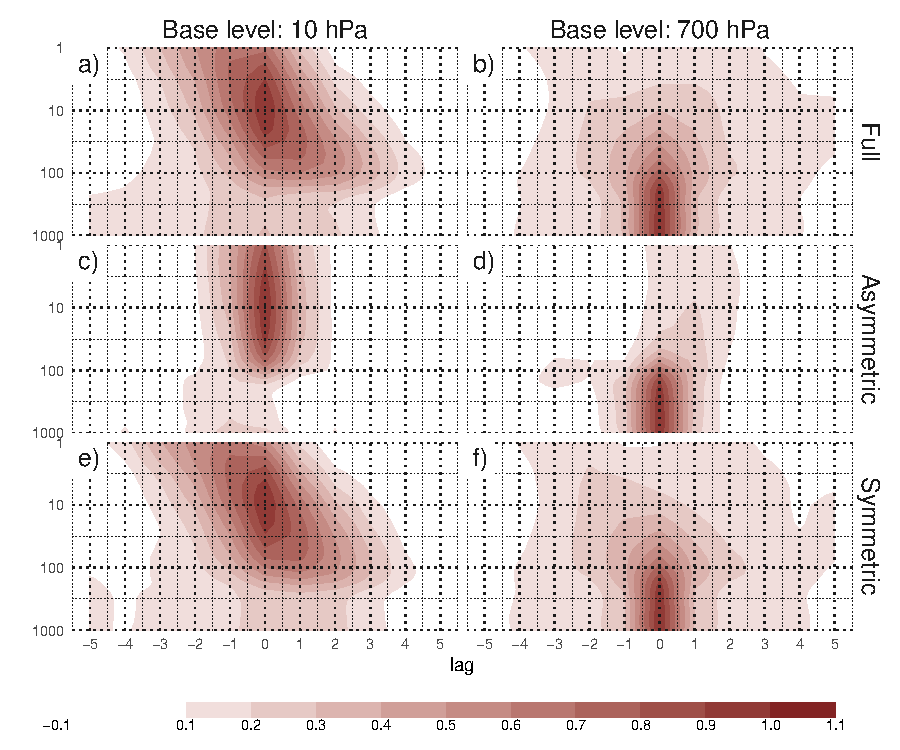
\includegraphics{A2 ccf-levels-1} \caption[Cross-correlation functions for each index and two differnet base levels]{Cross-correlation functions for each index and two differnet base levels.}\label{fig:A2 ccf-levels}
\end{figure}

\begin{figure}
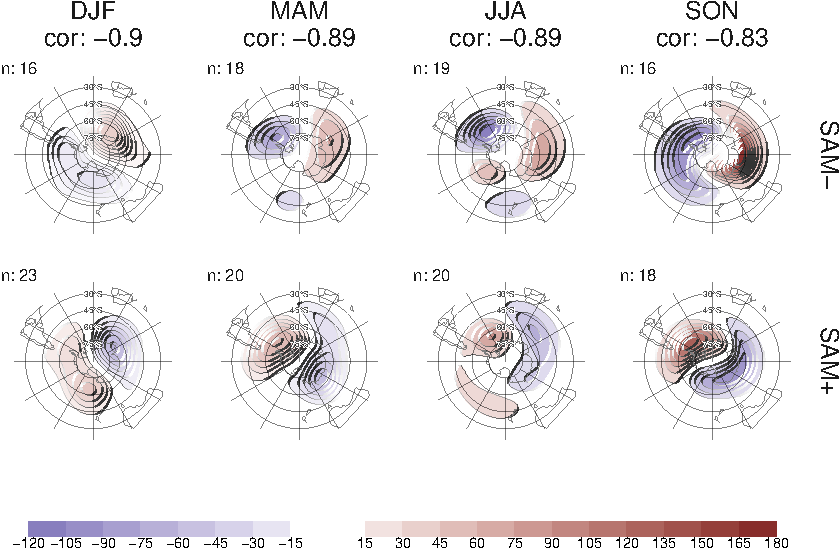
\includegraphics{A3-1} \appendcaption{A3}{Fourier spectrum of each timeseries. The shading indicates de 95\% area derived by fitting an AR process to each series and bootstrapping 5000 simulated samples.}\label{fig:A3}
\end{figure}

\begin{figure}
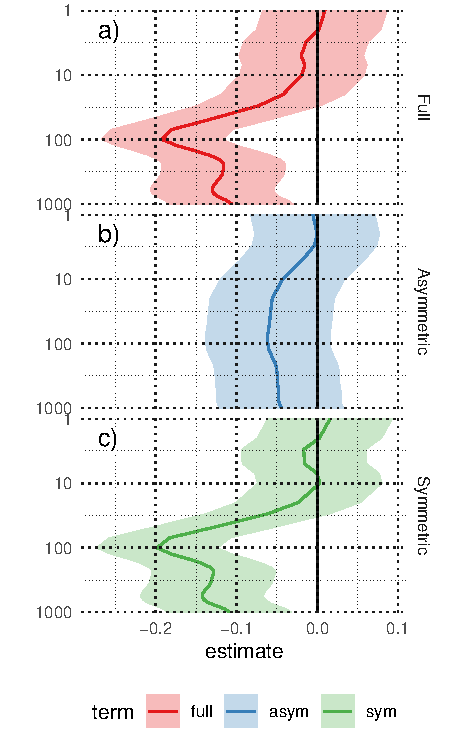
\includegraphics{A4-1} \appendcaption{A4}{Autocorrelation functions of each timeseries}\label{fig:A4}
\end{figure}

\begin{figure}
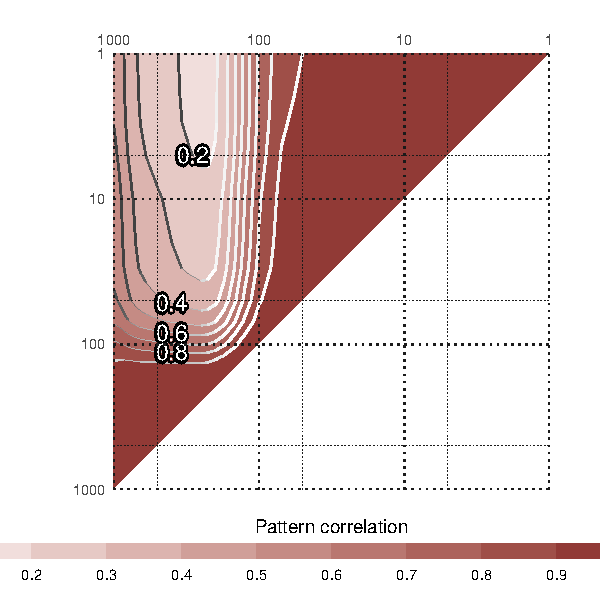
\includegraphics{A8-1} \appendcaption{A8}{Pattern cross-correlation \#FIXME!}\label{fig:A8}
\end{figure}

\begin{figure}
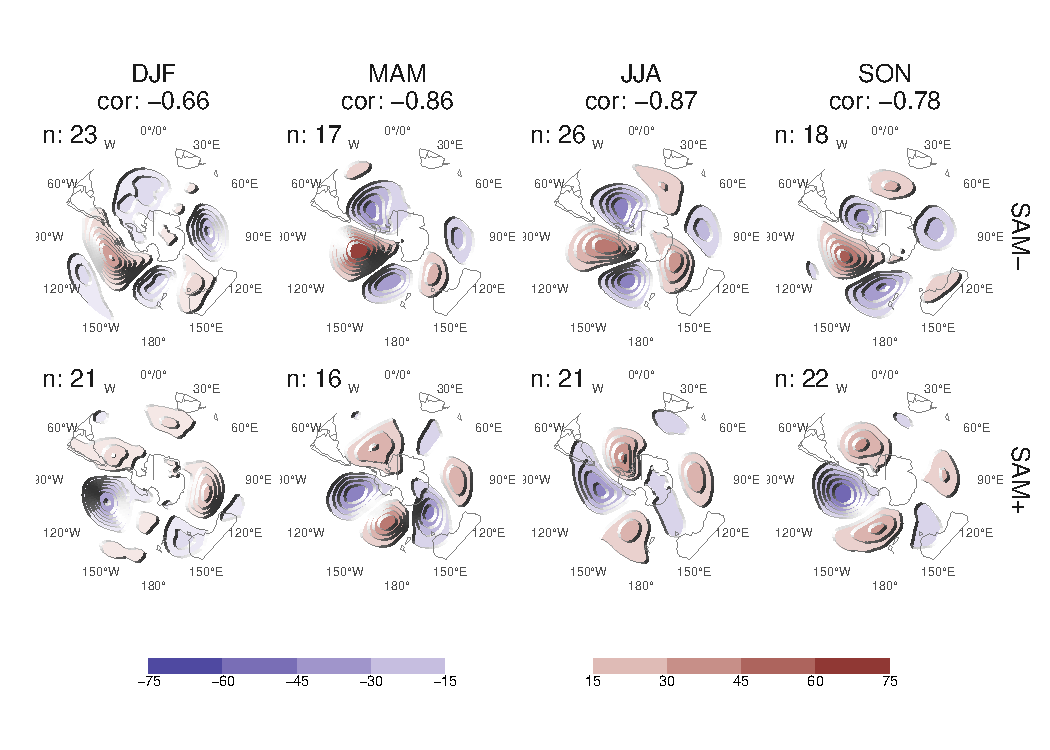
\includegraphics{A9-1} \caption[700 hPa Geopotetnial height zonal anomalies of composites of positive and negative SAM months selected using 1 standard deviation as threshhold]{700 hPa Geopotetnial height zonal anomalies of composites of positive and negative SAM months selected using 1 standard deviation as threshhold. Numbers in the column headers are pattern correlation between SAM+ and SAM- composites and number of monthly fields used to construct the composites.}\label{fig:A9}
\end{figure}

\begin{figure}
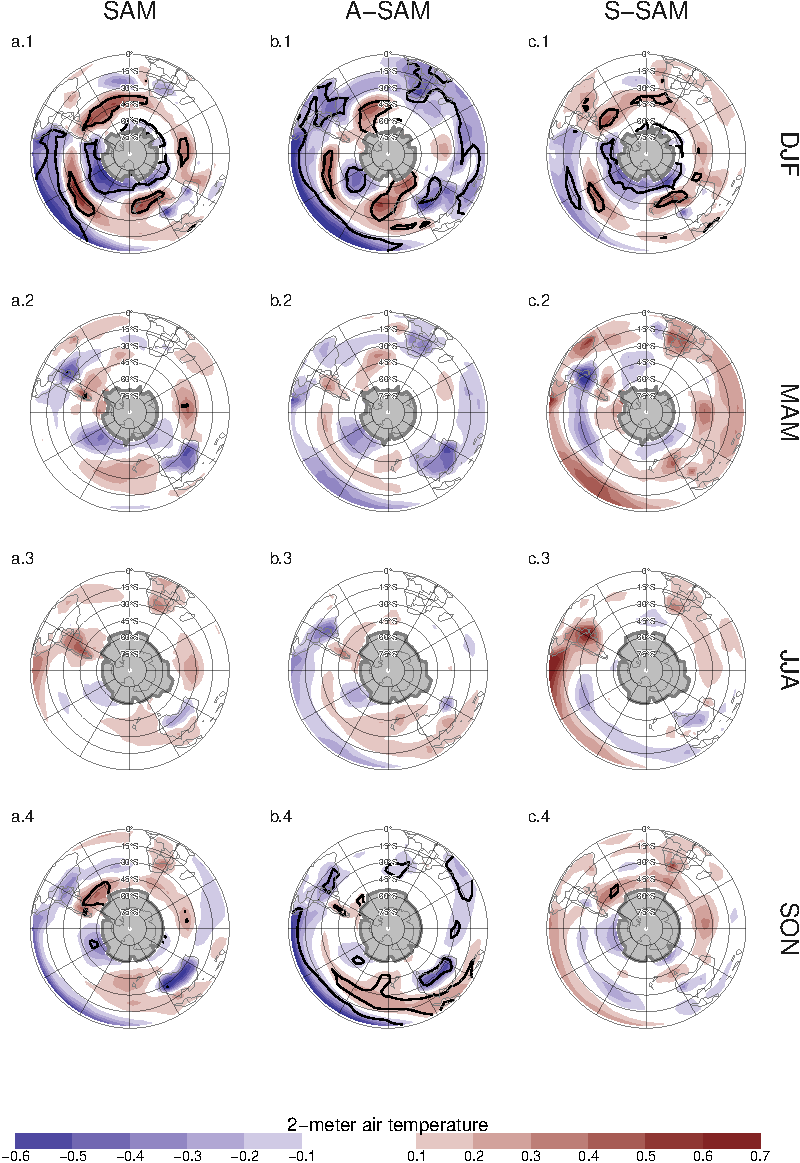
\includegraphics{A10-1} \caption[Zonal of projection of 700 hPa onto the first EOF of each season]{Zonal of projection of 700 hPa onto the first EOF of each season.}\label{fig:A10}
\end{figure}


\end{document}
